%% LyX 2.1.2 created this file.  For more info, see http://www.lyx.org/.
%% Do not edit unless you really know what you are doing.
\documentclass[11pt,english]{article}
\renewcommand{\rmdefault}{cmr}
\renewcommand{\sfdefault}{cmss}
\renewcommand{\ttdefault}{cmtt}
\usepackage[T1]{fontenc}
\usepackage[latin9]{inputenc}
\usepackage{geometry}
\geometry{verbose,tmargin=2.5cm,bmargin=2.5cm,lmargin=2.5cm,rmargin=2.5cm}
\setlength{\parskip}{\bigskipamount}
\setlength{\parindent}{0pt}
\usepackage{babel}
\usepackage{float}
\usepackage{amsthm}
\usepackage{amsmath}
\usepackage{amssymb}
\usepackage{esint}
\usepackage[unicode=true,pdfusetitle,
 bookmarks=true,bookmarksnumbered=false,bookmarksopen=false,
 breaklinks=false,pdfborder={0 0 0},backref=false,colorlinks=false]
 {hyperref}

\makeatletter
%%%%%%%%%%%%%%%%%%%%%%%%%%%%%% Textclass specific LaTeX commands.
\theoremstyle{plain}
\newtheorem{thm}{\protect\theoremname}[section]
  \theoremstyle{definition}
  \newtheorem{defn}[thm]{\protect\definitionname}
  \theoremstyle{remark}
  \newtheorem{rem}[thm]{\protect\remarkname}
  \theoremstyle{plain}
  \newtheorem{lem}[thm]{\protect\lemmaname}

%%%%%%%%%%%%%%%%%%%%%%%%%%%%%% User specified LaTeX commands.
\let\originalleft\left
\let\originalright\right
\renewcommand{\left}{\mathopen{}\mathclose\bgroup\originalleft}
\renewcommand{\right}{\aftergroup\egroup\originalright}
\usepackage{pgfplots}
\usetikzlibrary{pgfplots.groupplots}
\usepackage{verbatim}

\usetikzlibrary{external}
\tikzexternalize

\newcounter{fakelem}

\makeatletter
\renewcommand*{\UrlTildeSpecial}{%
  \do\~{%
    \mbox{%
      \fontfamily{ptm}\selectfont
      \textasciitilde
    }%
  }%  
}%    
\let\Url@force@Tilde\UrlTildeSpecial
\makeatother

\makeatletter
\@addtoreset{fakelem}{enumi}
\makeatother

\usepackage{enumitem}
\setlist[enumerate]{itemsep=15pt}

\newenvironment{question}
%{\expandafter\comment}
%{\expandafter\endcomment}
{\itshape}
{\par\vspace{10pt}}

\newcommand{\displaycompensate}{}%\vspace{-15pt}}

%graph drawing
\usepackage{tikz}
\usetikzlibrary{decorations.markings}
\usetikzlibrary{arrows.meta}
\tikzstyle{vertex}=[circle,draw=black,fill=black,inner sep=0,minimum size=0.2cm,text=white,font=\footnotesize]
\tikzset{arc/.style={
        decoration={markings,
            mark= at position 0.5 with {\arrow{Latex[length=2mm,width=2mm]}} ,
        },
        postaction={decorate}
    }
}
\tikzset{every loop/.style={min distance=50,in=50,out=130,looseness=7}}

\usepackage[labelfont=bf,labelsep=period]{caption}

\makeatother

  \providecommand{\definitionname}{Definition}
  \providecommand{\lemmaname}{Lemma}
  \providecommand{\remarkname}{Remark}
\providecommand{\theoremname}{Theorem}

\begin{document}

\title{Discrete Smoothed Analysis}


\author{Matthew Kwan}

\maketitle
\global\long\def\RR{\mathbb{R}}


\global\long\def\QQ{\mathbb{Q}}


\global\long\def\HH{\mathbb{H}}


\global\long\def\E{\mathbb{E}}


\global\long\def\Var{\operatorname{Var}}


\global\long\def\CC{\mathbb{C}}


\global\long\def\NN{\mathbb{N}}


\global\long\def\ZZ{\mathbb{Z}}


\global\long\def\GG{\mathbb{G}}


\global\long\def\BB{\mathbb{B}}


\global\long\def\DD{\mathbb{D}}


\global\long\def\cL{\mathcal{L}}


\global\long\def\supp{\operatorname{supp}}


\global\long\def\one{\boldsymbol{1}}


\global\long\def\range#1{\left[#1\right]}


\global\long\def\d{\operatorname{d}}


\global\long\def\falling#1#2{\left(#1\right)_{#2}}


\global\long\def\f{\mathbf{f}}


\global\long\def\im{\operatorname{im}}


\global\long\def\sp{\operatorname{span}}


\global\long\def\sign{\operatorname{sign}}


\global\long\def\mod{\operatorname{mod}}


\global\long\def\id{\operatorname{id}}


\global\long\def\disc{\operatorname{disc}}


\global\long\def\lindisc{\operatorname{lindisc}}


\global\long\def\tr{\operatorname{tr}}


\global\long\def\adj{\operatorname{adj}}


\global\long\def\Unif{\operatorname{Unif}}


\global\long\def\Po{\operatorname{Po}}


\global\long\def\Bin{\operatorname{Bin}}


\global\long\def\Ber{\operatorname{Ber}}


\global\long\def\Geom{\operatorname{Geom}}


\global\long\def\Hom{\operatorname{Hom}}


\global\long\def\floor#1{\left\lfloor #1\right\rfloor }


\global\long\def\ceil#1{\left\lceil #1\right\rceil }


\global\long\def\T{\mathbf{T}}


\global\long\def\N{\mathbf{N}}


\global\long\def\B{\mathbf{B}}


\global\long\def\a{\boldsymbol{\alpha}}


\global\long\def\b{\boldsymbol{\beta}}


\global\long\def\x{\mathbf{x}}


\global\long\def\y{\mathbf{y}}


\global\long\def\o{\boldsymbol{\omega}}



\section{Perfect Matchings and Hamilton Cycles in Hypergraphs}

For hypergraphs, there is no single most natural notion of ``minimum
degree''.
\begin{defn}
Let $H$ be a $k$-uniform hypergraph. The \emph{degree} of a set
of vertices $s\subseteq V\left(H\right)$ is the number of hyperedges
that include $s$. The \emph{minimum $q$-degree} $\delta_{q}\left(H\right)$
of $H$ is the minimum degree among all $s\subseteq V\left(H\right)$
with $\left|s\right|=q$.\end{defn}
\begin{rem}
\label{rem:hypergraph-degree-transfer}We say graphs are dense if
they have many edges (have large $\delta_{0}$), or more strongly
if they have large minimum degree (have large $\delta_{1}$). The
idea of minimum $q$-degree generalizes this for hypergraphs. Indeed,
for a $k$-regular hypergraph $H$, a double-counting argument shows
that if $q\le p$ then 
\[
\delta_{q}\left(H\right)\ge\delta_{p}\left(H\right){n-q \choose p-q}\left.\vphantom{\sum}\right/{k-q \choose p-q}.
\]
So, imposing that a $k$-uniform hypergraph has large $\left(k-1\right)$-degree
ensures that it has large $q$-degrees for all $q$.\end{rem}
\begin{defn}
Let $\HH_{k}\left(n,m\right)$ be the random $k$-uniform hypergraph
on the vertex set $\left[n\right]$ chosen uniformly from all 3-uniform
hypergraphs with $m$ hyperedges.
\end{defn}
The purpose of this section is to prove the following two theorems.
\begin{thm}
\label{thm:hypergraph-perfect-matching}There is $\beta_{k}\left(\alpha\right)$
such that if $H$ is a $k$-uniform hypergraph on $\left[kn\right]$
with $\delta_{k-1}\left(H\right)\ge\alpha n$, and $R\in\HH\left(kn,\beta_{k}\left(\alpha\right)n\right)$,
then $H\cup R$ a.a.s. has a perfect matching.
\end{thm}

\begin{thm}
\label{thm:hypergraph-hamiltonian}There is $\gamma_{k}\left(\alpha\right)$
such that if $H$ is a $k$-uniform hypergraph on $\left[\left(k-1\right)n\right]$with
$\delta_{k-1}\left(H\right)\ge\alpha n$, and $R\in\HH\left(\left(k-1\right)n,\gamma_{k}\left(\alpha\right)n\right)$,
then $H\cup R$ a.a.s. has a loose Hamilton cycle.\end{thm}
\begin{rem}
\label{rem:large-degrees-all-orders}By Remark \ref{rem:hypergraph-degree-transfer},
our requirement $\delta_{k-1}\left(H\right)=\Omega\left(n\right)$
actually implies $\delta_{q}\left(H\right)=\Omega\left(n^{k-q}\right)$
for all $q$. We do not know whether such requirements on the $q$-degrees
with $q<k-1$ suffice for the conclusions of our theorems. I NEED
TO THINK ABOUT THIS.
\end{rem}

\subsection{Proofs of Theorems \ref{thm:hypergraph-perfect-matching} and \ref{thm:hypergraph-hamiltonian}}

Our theorems will follow from a sequence of lemmas. The first step
is to show that $R$ almost gives the structure of interest on its
own. Let a\emph{ sub-cycle} be a hypergraph which can be extended
to a loose Hamilton cycle by adding edges.
\begin{lem}
\label{lem:large-hypergraph-matching}For any $\varepsilon>0$, there
is $\beta_{k}'\left(\varepsilon\right)$ such that a random hypergraph
distributed as $\HH_{k}\left(kn,\beta_{k}'\left(\varepsilon\right)\right)$
a.a.s. has a matching of size $\left(1-\varepsilon\right)n$.
\end{lem}

\begin{lem}
\label{lem:large-hypergraph-subcycle}For any $\varepsilon>0$, there
is $\gamma_{k}'\left(\varepsilon\right)$ such that a random hypergraph
distributed as $\HH_{k}\left(\left(k-1\right)n,\gamma_{k}'\left(\varepsilon\right)\right)$
a.a.s. has a sub-cycle of size $\left(1-\varepsilon\right)n$.\end{lem}
\begin{proof}
[Proof of Lemma \ref{lem:large-hypergraph-matching}]To realize the
distribution $\HH_{k}\left(kn,\beta_{k}'\left(\varepsilon\right)n\right)$,
imagine that independently uniformly random hyperedges are repeatedly
dropping into $R$, until we have seen $\beta_{k}'\left(\varepsilon\right)$
distinct hyperedges. We iteratively build a matching $M$ greedily.
If a new hyperedge $e$ drops into $R$ which does not share any vertices
with the hyperedges in $M$ so far, then add $e$ to $M$. If we have
already added $i$ hyperedges to $M$, then the probability we will
add the next random hyperedge is
\[
p_{i}={kn-ki \choose k}\left.\vphantom{\sum}\right/{kn \choose k}=\Omega\left(\left(\frac{n-i}{n}\right)^{k}\right).
\]
The number of random edges required to build a matching of size $\left(1-\varepsilon\right)n$
therefore has the distribution of
\[
X=\sum_{i=1}^{\left(1-\varepsilon\right)n}X_{i},
\]
where each $X_{i}$ is independently geometrically distributed with
success probability $p_{i}$. By Chebyshev's inequality or a Chernoff
bound, $X$ is a.a.s. close to its expectation, which is at most 
\[
O\left(\sum_{i=1}^{\left(1-\varepsilon\right)n}n^{k}/\left(n-i\right)^{k}\right)=O\left(n^{k}\int_{\varepsilon n}^{\infty}\frac{1}{x^{k}}dx\right)=O\left(n\right).
\]
So, if $\beta_{k}'\left(\varepsilon\right)$ is large enough then
a.a.s. $\left|M\right|\ge\left(1-\varepsilon\right)n$.
\end{proof}

\begin{proof}
[Proof of Lemma \ref{lem:large-hypergraph-subcycle}]A sub-cycle is
a loose Hamilton cycle or a disjoint union of loose paths, but a union
of disjoint paths may not be a sub-cycle if it has so many paths that
there are not enough vertices left to link them together. A union
of $j$ paths (which have length greater than zero) with a total of
$i$ hyperedges is a sub-cycle precisely when $i+j\le n$. Call such
sub-cycles \emph{proper }sub-cycles.

As in the proof of \ref{lem:large-hypergraph-matching}, imagine that
independently uniformly random hyperedges are repeatedly dropping
into $R$. We build a proper sub-cycle $S$ greedily. Suppose we are
at a point where $S$ has $i$ hyperedges and $j$ paths, with $i\le\left(1-\varepsilon\right)n$.
There are $\left(k-1\right)i+j\le\left(k-2\right)i+n$ vertices in
the paths in $S$. 

There are 3 kinds of hyperedges we can add to $S$: a hyperedge that
starts a new loose path (``type 1''), a hyperedge that extends an
existing path (``type 2''), or a hyperedge that joins two paths
together (``type 3''). We can only add a type 1 hyperedge when $i+j\le n-2$,
and can only add a type 2 hyperedge when $i+j\le n-1$.

If $i+j\le n-2$ then there are at least 
\[
{\left(k-1\right)n-\left(\left(k-2\right)i+n\right) \choose k}={\left(k-2\right)\left(n-i\right) \choose k}=\Omega\left(\left(n-i\right)^{k}\right)
\]
type-1 hyperedges that could possibly be added. Otherwise, we must
have $j>n-2-i\ge\varepsilon n-2$, so (identifying one vertex in an
extremal hyperedge of each path as ``eligible to be joined''), there
are at least 
\[
{j \choose 2}{\left(k-2\right)\left(n-i\right) \choose k-2}=\Omega\left(n^{2}\left(n-i\right)^{k-2}\right)=\Omega\left(\left(n-i\right)^{k}\right)
\]
type-3 hyperedges that could be added. Combining both cases, we can
see that if $S$ has $i\le\left(1-\varepsilon\right)n$ hyperedges,
then the next edge will be added with probability at least
\[
\Omega\left(\left(n-i\right)^{k}\right)\left.\vphantom{\sum}\right/{\left(k-1\right)n \choose k}=\Omega\left(\left(\frac{n-i}{n}\right)^{k}\right).
\]
We conclude with the same reasoning as the proof of Lemma \ref{lem:large-hypergraph-matching}.
\end{proof}
The second step to prove Theorems \ref{thm:hypergraph-perfect-matching}
and \ref{thm:hypergraph-hamiltonian} is to show that a dense hypergraph
plus a large partial structure a.a.s. gives the structure we are looking
for. For both theorems, we will be able to reduce this step to the
following lemma.
\begin{lem}
\label{lem:bipartite-plus-big-matching-perfect}There is $\xi\left(\alpha\right)>0$
such that the following holds. Let $G$ be a bipartite graph with
partitions $A,B$ of equal size $n$, and suppose $\delta\left(G\right)\ge\alpha n$.
Let $M$ be a uniformly random matching with $\left(1-\xi\left(\alpha\right)\right)n$
edges between $A$ and $B$. Then $G\cup M$ has a perfect matching.\end{lem}
\begin{proof}
We use Hall's marriage theorem: we need to show that a.a.s. $\left|N_{G\cup M}\left(W\right)\right|\ge\left|W\right|$
for all $W\subseteq A$. If $\left|W\right|\le\alpha n$, then $\left|N_{G\cup M}\left(W\right)\right|\ge\left|N_{G}\left(W\right)\right|\ge\alpha n\ge\left|W\right|$
by the degree condition on $G$. Similarly, if $\left|W\right|\ge\left(1-\alpha\right)n$
then every $b\in B$ has an edge to $W$ in $G$, so $\left|N_{G\cup M}\left(W\right)\right|=\left|B\right|\ge\left|W\right|$.
The difficult case is where $\alpha n\le\left|W\right|\le\left(1-\alpha\right)n$.
It is relatively straightfoward to prove that for any individual such
$W$, a.a.s. $\left|N_{G\cup M}\left(W\right)\right|\ge\left|W\right|$.
However the probability of failure is not small enough for a union
bound over all choices of $W$. Our approach is to use Szemer\'edi's
regularity lemma on $G$ and to show that the random matching a.a.s.
distributes very evenly over the resulting clusters. Then, $\varepsilon$-regularity
and the even distribution of the added edges are enough to ensure
that $\left|N_{G\cup M}\left(W\right)\right|\ge\left|W\right|$ for
each $W$.

We use a bipartite version of Szemer\'edi's regularity lemma (which
can be deduced from say \cite[Theorem 2.3]{Tao05} in a similar way
to \cite[Theorem 1.10]{KS96}). Let $\alpha'=\alpha/2$ and let $\varepsilon>0$
be a small constant depending on $\alpha$ that will be determined
later (assume for now that $\varepsilon<\alpha/8$). There is a large
constant $K$ depending only on $\alpha$ such that there exist partitions
$A=V_{0}^{1}\cup\dots\cup V_{k}^{1}$ and $B=V_{0}^{2}\cup\dots\cup V_{k}^{2}$
with $k\le K$, in such a way that the following conditions are satisfied.
The ``exceptional'' clusters $V_{0}^{1}$ and $V_{0}^{2}$ both
have fewer than $\varepsilon n$ vertices, and the non-exceptional
clusters in $A$ and $B$ have equal size: $\left|V_{1}^{1}\right|=\dots=\left|V_{k}^{\ell}\right|=an$
and $\left|V_{1}^{1}\right|=\dots=\left|V_{k}^{\ell}\right|=bn$.
There is a subgraph $G'\subseteq G$ with minimum degree at least
$\left(\alpha'+\varepsilon\right)n$ such that each pair of distinct
clusters $V_{i}^{1},V_{j}^{2}$ ($i,j\ge1$) is $\varepsilon$-regular
in $G'$ with density zero or at least $2\varepsilon$. Define the
cluster graph $\mathfrak{G}$ as the bipartite graph whose vertices
are the non-exceptional clusters $V_{i}^{\ell}$, and whose edges
are the pairs of clusters between which there is nonzero density in
$G'$.

Fix some $V_{i}^{1}$ and $V_{j}^{2}$, with $i,j\ge1$. The vertices
of each $V_{i}^{1}$ are matched by $M$ to at most $an$ vertices;
conditioning on their number, they are uniformly randomly chosen from
$B$. Let $X_{b}$ be the indicator random variable for the event
that the vertex $b\in B$ is matched with a vertex in $V_{i}^{1}$.
The random variables $X_{b}$ are said to be \emph{negatively associated}
(see \cite[Application 3.1(c)]{JDP83}). This means in particular
that we can apply Chernoff bounds to $\sum_{b\in V_{j}^{2}}X_{b}$
even though the $X_{b}$ are not independent. By a union bound, a.a.s.
there are at most $\left(ab+\xi\left(\alpha\right)\right)n$ edges
of $M$ between every pair $V_{i}^{1}$, $V_{j}^{2}$. We assume this
holds for the remainder of the proof.

Now, in $G'$ each $V_{i}^{\ell}$ has at least $\left(\alpha'+\varepsilon\right)n\left|V_{i}^{\ell}\right|$
edges to other clusters. There are at most $\varepsilon n\left|V_{i}^{\ell}\right|$
edges to the exceptional cluster $V_{0}$ and at most $\left|V_{i}^{\ell}\right|^{2}$
edges to each other cluster. So, $d_{\mathfrak{G}}\left(V_{i}^{\ell}\right)\ge\left(\left(\beta+\varepsilon\right)n\left|V_{i}^{\ell}\right|-\varepsilon n\left|V_{i}^{\ell}\right|\right)/\left|V_{i}^{\ell}\right|^{2}\ge\alpha'k$
and $\mathfrak{G}$ has minimum degree at least $\alpha'k$.

Consider any $W\subset A$ with $\alpha n\le\left|W\right|\le\left(1-\alpha\right)n$.
For each $i$ let $\pi_{i}=\left|V_{i}^{1}\cap W\right|/\left(an\right)$,
and let $\mathfrak{H}$ be the set of clusters $V_{i}^{1}$ with $\pi_{i}\ge\varepsilon$.
If $\varepsilon$ is small, $\mathfrak{H}$ must be nonempty. Now,
if $V_{j}^{2}\in N_{\mathfrak{G}}\left(\mathfrak{H}\right)$ then
by $\varepsilon$-regularity there are edges in $G'$ from $W$ to
at least $\left(1-\varepsilon\right)bn$ vertices of $V_{j}^{2}$.
It follows that if $\left|N_{\mathfrak{G}}\left(\mathfrak{H}\right)\right|=k$
(that is, every $V_{i}^{\ell}$ is a neighbour of $\mathfrak{H}$)
then $\left|N_{G\cup M}\left(W\right)\right|\ge\left|N_{G'}\left(W\right)\right|\ge\left(1-\varepsilon\right)\left(n-\left|V_{0}^{2}\right|\right)\ge\left|W\right|$
for small $\varepsilon$, and we are done.

Otherwise, choose $\mathfrak{S}\subseteq N\left(\mathfrak{H}\right)$
with $\left|\mathfrak{S}\right|=\alpha'k$ and let $S$ be the vertices
in the clusters of $\mathfrak{S}$. By the same $\varepsilon$-regularity
argument, $\left|N_{G'}\left(W\right)\cap S\right|\ge\alpha'k\left(1-\varepsilon\right)bn\ge\left(1-\varepsilon\right)^{2}\alpha'n$.
We are assuming there is $V_{j}^{2}$ outside $N_{\mathfrak{G}}\left(\mathfrak{H}\right)$,
and this $V_{j}^{2}$ must have $\alpha'k$ neighbours outside $\mathfrak{H}$
in $\mathfrak{G}$, so $\left|\mathfrak{H}\right|\le\left(1-\alpha'\right)k$.
Since $\left|M\right|=\left(1-\xi\left(\alpha\right)\right)n$, each
$V_{i}^{1}\cap W$ has at least $\left(\pi_{i}a-\xi\left(\alpha\right)\right)n$
neighbours in $M$, and at most $\alpha'k\left(ab+\xi\left(\alpha\right)\right)n$
of these are in $S$. So, 
\begin{align*}
\left|N_{M}\left(W\right)\backslash S\right| & \ge\sum_{V_{i}^{1}\in\mathfrak{H}}\left(\pi_{i}a-\xi\left(\alpha\right)\right)n-\left|\mathfrak{H}\right|\left(\alpha'k\left(ab+\xi\left(\alpha\right)\right)\right)n\\
 & \ge\left|W\right|-\varepsilon n-\left(1-\alpha'\right)\alpha'\left(1-\varepsilon\right)^{2}-k^{2}\xi\left(\alpha\right)n
\end{align*}
and
\[
\left|N_{G\cup M}\left(W\right)\right|\ge\left|W\right|+\left(\alpha'\left(1-\varepsilon\right)^{2}-\varepsilon-\left(1-\alpha'\right)\alpha'\left(1-\varepsilon\right)^{2}-k^{2}\xi\left(\alpha\right)\right)n.
\]


If $\varepsilon$ is chosen to be small enough relative to $\alpha$
and $\xi\left(\alpha\right)$ chosen to be small enough relative to
$K$, then this gives $\left|N_{G\cup M}\left(W\right)\right|\ge\left|W\right|$.
\end{proof}
Now we describe the reduction of Theorems \ref{thm:hypergraph-perfect-matching}
and \ref{thm:hypergraph-hamiltonian} to Lemma \ref{lem:bipartite-plus-big-matching-perfect}.
Consider a $k$-uniform hypergraph $H$. Suppose $A$ is a set of
$n$ vertices and $B$ is a $\left(k-1\right)$-uniform hypergraph
on the remaining vertices. Then we define a bipartite graph $G_{A,B}\left(H\right)$
as follows. The vertices of $G_{A,B}\left(H\right)$ are the vertices
in $A$, as well as the edges in $B$ (we abuse notation and identify
the hypergraph $B$ with its edge set). We put an edge between $a\in A$
and $\left\{ b_{1},\dots,b_{k-1}\right\} \in B$ if $\left\{ a,b_{1},\dots,b_{k-1}\right\} $
is a hyperedge in $H$.

The significance of $G_{A,B}\left(H\right)$ is that if $B$ is a
perfect matching or loose Hamilton cycle on $V\left(H\right)\backslash A$,
and if $G_{A,B}\left(H\right)$ has a large matching $M$, then the
edges of $M$ correspond to a large matching (respectively, a large
sub-cycle) in $H$. Conversely, if $H$ has a large matching or Hamilton
cycle (as provided by Lemmas \ref{lem:large-hypergraph-matching}
and \ref{lem:large-hypergraph-subcycle}), then there is a set $A$
and a perfect matching (respectively, loose Hamilton cycle) $B$ such
that $G_{A,B}\left(H\right)$ has a large matching.

By the symmetry of the distribution of $R$, we can assume $A$ and
$B$ are uniformly random. We give one final pair of lemmas, ensuring
that the linear minimum $\left(k-1\right)$-degree of $H$ corresponds
a.a.s. to linear minimum degree in $G_{A,B}\left(H\right)$.
\begin{lem}
\label{lem:matching-degree-transfer}There is $\eta\left(\alpha\right)>0$
such that the following holds. Let $H$ satisfy the conditions of
Theorem \ref{thm:hypergraph-perfect-matching}, let $A$ be a uniformly
random set of $n$ vertices, and let $B$ be a uniformly random perfect
matching on $V\left(H\right)\backslash A$. Then a.a.s. $G_{A,B}\left(H\right)$
has minimum degree $\eta\left(\alpha\right)n$.
\end{lem}

\begin{lem}
\label{lem:hamilton-degree-transfer}There is $\zeta\left(\alpha\right)>0$
such that the following holds. Let $H$ satisfy the conditions of
Theorem \ref{thm:hypergraph-hamiltonian}, let $A$ be a uniformly
random set of $n$ vertices, and let $B$ be a uniformly random loose
Hamilton cycle on $V\left(H\right)\backslash A$. Then a.a.s. $G_{A,B}\left(H\right)$
has minimum degree $\zeta\left(\alpha\right)n$.\end{lem}
\begin{proof}
[Proof of Lemma \ref{lem:matching-degree-transfer}]It is helpful
to conceptualize the randomness in a certain way. Let 
\[
a_{1},\dots,a_{n},\, b_{1}^{1},\dots,b_{k}^{1},\, b_{1}^{2},\dots,b_{k}^{n}
\]
be a uniformly random ordering of $V\left(H\right)$. Let $A=\left\{ a_{1},\dots,a_{n}\right\} $,
let $b^{i}=\left\{ b_{1}^{i},\dots,b_{k}^{i}\right\} $ and let $B=\left\{ b^{1},\dots,b^{n}\right\} $.

First, condition on some $b=b^{i}$. Note that $\Pr\left(b\cup\left\{ a_{1}\right\} \in E\left(H\right)\right)\ge\delta_{k-1}\left(H\right)/n$
and more generally
\[
\Pr\left(b\cup\left\{ a_{j}\right\} \in E\left(H\right)\mid a_{1},\dots,a_{j}\right)\ge\left(\delta_{k-1}\left(H\right)-j\right)/n\ge\alpha/2
\]
for $j\le\alpha n/2$. By a Chernoff bound, $d_{G_{H}}\left(b\right)\ge\alpha^{2}n/8$
with probability $1-e^{-\Omega\left(n\right)}$. With a union bound,
this a.a.s. holds for all $b$.

Now, recall from Remark \ref{rem:large-degrees-all-orders} that $\delta_{1}\left(H\right)\ge\alpha'n^{k-1}$
for some $\alpha'$ depending on $\alpha$. Condition on some $a=a_{i}$.
Each $b_{j}^{i}$ shares at most ${n \choose k-2}$ hyperedges with
$a_{i}$, so if $j\le2\sqrt{\eta\left(\alpha\right)}n$ for sufficently
small $\eta\left(\alpha\right)$ and large $n$, then 
\[
\Pr\left(\left\{ a\right\} \cup b^{j+1}\in E\left(H\right)\mid b^{1},\dots,b^{j}\right)\ge\left(\delta_{1}\left(H\right)-kj{n \choose k-2}\right)\left.\vphantom{\sum}\right/{n \choose k-1}\ge\sqrt{\eta\left(\alpha\right)}.
\]


By a Chernoff bound and a union bound, a.a.s. each $d_{G_{H}}\left(a\right)\ge\eta\left(\alpha\right)$.
\end{proof}

\begin{proof}
[Proof of Lemma \ref{lem:hamilton-degree-transfer}]We give essentially
the same proof as for Lemma \ref{lem:matching-degree-transfer}. Let
\[
a_{1},\dots,a_{n},b_{0},\dots,b_{\left(k-2\right)n-1}
\]
be a uniformly random ordering of $V\left(H\right)$. Let $A=\left\{ a_{1},\dots,a_{n}\right\} $,
let $b^{i}=\left\{ b_{\left(k-2\right)i},b_{\left(k-2\right)i+1},\dots,b_{\left(k-2\right)\left(i+1\right)}\right\} $
(where the subscripts are interpreted modulo $\left(k-2\right)n$),
and let $B=\left\{ b^{1},\dots,b^{n}\right\} $.

With exactly the same proof as for \ref{lem:matching-degree-transfer},
there is small $\zeta\left(\alpha\right)$ such that a.a.s. $d_{G_{H}}\left(b\right)\ge\zeta\left(\alpha\right)n$
for all $b$. Next, condition on some $a=a_{i}$. For small $\zeta\left(\alpha\right)$
and $j\le2\sqrt{\zeta\left(\alpha\right)}n$, 
\[
\Pr\left(\left\{ a\right\} \cup b^{j}\in E\left(H\right)\mid b^{0},\dots,b^{j-1}\right)\ge\left(\delta_{2}\left(H\right)-\left(k-2\right)j{n \choose k-3}\right)\left.\vphantom{\sum}\right/{n \choose k-2}\ge\sqrt{\zeta\left(\alpha\right)},
\]


so a.a.s. each $d_{G_{H}}\left(a\right)\ge\zeta\left(\alpha\right)n$.
\end{proof}
We have established that $G_{A,B}\left(H\right)$ is a bipartite graph
with linear minimum degree. If we condition on $A$ and $B$, then
$G_{A,B}\left(R\right)$ a.a.s. provides a uniformly random large
matching between $A$ and $B$, so Lemma \ref{lem:bipartite-plus-big-matching-perfect}
ensures the existence of a perfect matching in $G_{A,B}\left(H\cup R\right)$,
corresponding to a perfect matching or loose Hamilton cycle in $H\cup R$.


\section{Hamiltonicity in dense digraphs}

MOTIVATION, BACKGROUND, DEFINITIONS AND EQUIVALENCE OF MODELS TO COME
LATER.

It was observed by Bondy \cite{Bon75} that almost any non-trivial
condition on a graph $G$ that ensures the existence of a Hamilton
cycle also ensures the existence of cycles of all lengths ranging
from 3 to $\left|G\right|$ (we say such a graph is \emph{pancyclic}).
In \cite{BFM03}, the authors proved that adding a sufficiently large
linear number of edges to a dense graph or digraph a.a.s. ensures
the existence of a Hamilton cycle. In accordance with Bondy's observation,
we prove the following theorem. (Note that the corresponding result
for undirected graphs is an immediate corollary).
\begin{thm}
\label{thm:smoothed-pancyclic}For each $\alpha>0$, there is $\beta\left(\alpha\right)$
such that the following holds. Let $D$ be digraph on $n$ vertices
with minimum (in- and out-) degree $\alpha n$. Uniformly at random,
choose $\beta\left(\alpha\right)n$ arcs not already in $D$ and add
them to $D$. The resulting digraph $D'$ is a.a.s. pancyclic.
\end{thm}
The proofs in \cite{BFM03} can give an exponentially small bound
on the probability of failure to be Hamiltonian, so it is possible
to use a union bound and some small adjustments to prove Theorem \ref{thm:smoothed-pancyclic}
as a corollary. However, we prefer to give an alternative proof, which
we feel is more direct. The key to our proof is the following lemma,
which gives a very general condition for pancyclicity based on an
expansion property.
\begin{lem}
\label{lem:pseudorandom-pancyclic}Let $D$ be a directed graph on
$n$ vertices with $\delta\left(D\right)\ge8k$, and suppose for all
disjoint $A,B\subseteq V\left(D\right)$ with $\left|A\right|=\left|B\right|\ge k$,
there is an arc from $A$ to $B$. Then $D$ is pancyclic.
\end{lem}
Lemma \ref{lem:pseudorandom-pancyclic} will be a corollary of the
following lemma.
\begin{lem}
\label{lem:pseudorandom-hamiltonian}Let $D$ be a directed graph
with $\delta\left(D\right)\ge4k$, and suppose for all disjoint $A,B\subseteq V\left(D\right)$
with $\left|A\right|=\left|B\right|\ge k$, there is an arc from $A$
to $B$. Then $D$ is Hamiltonian.\end{lem}
\begin{rem}
\label{rem:constants}We have made no attempt to optimize the constant
in the degree condition of Lemma \ref{lem:pseudorandom-pancyclic}.
The ideas in the proof of Lemma \ref{lem:pseudorandom-hamiltonian}
can be used directly to prove Lemma \ref{lem:pseudorandom-pancyclic}
with a weaker condition on $\delta\left(D\right)$, but we do not
know whether the condition can be weakened all the way to $\delta\left(D\right)\ge4k$,
as Bondy's ``meta-conjecture'' would suggest. The constants in Lemmas
\ref{lem:pseudorandom-pancyclic} and \ref{lem:pseudorandom-hamiltonian}
can both be halved for the undirected case, just by simplifying the
main argument in the proof of Lemma \ref{lem:pseudorandom-hamiltonian}.\end{rem}
\begin{proof}
[Proof of Lemma \ref{lem:pseudorandom-hamiltonian}]The idea of the
proof is to start with a longest path $P$ and manipulate it into
a cycle $C$ on the same vertex set. We will show that $D$ is strongly
connected, so if $C$ were not Hamiltonian, there would be an arc
from $V\left(C\right)$ to its complement, which could be combined
with $C$ to give a longer path than $P$, contradicting maximality.

This type of argument goes back to a classical theorem by Dirac \cite[Theorem 3]{Dir52}.
It also bears some resemblance to the ``rotation-extension'' idea
introduced in \cite{Pos76}, and a variation for directed graphs in
\cite[Section 4.3]{FK05}.

First we acknowledge some immediate consequences of the condition
on $D$. Note that if $A$ and $B$ are disjoint sets with size at
least $k$, then in fact there are $\left|A\right|-k$ vertices of
$A$ with an arc into $B$. To see this, note that for any fewer number
of such vertices in $A$, we can delete those vertices and at least
$k$ will remain, one of which has an arc to $B$. Also, $D$ is strongly
connected. To see this, note that for any $v,w$, both of $N^{+}\left(v\right)$
and $N^{-}\left(w\right)$ have size at least $4k>k$. If they intersect
then there is a length-2 path from $v$ to $w$; otherwise there must
be an arc from $N^{+}\left(v\right)$ to $N^{-}\left(w\right)$ giving
a length-3 path.

Let $P=u\dots w$ be a maximal-length directed path in $D$. We will
use the notation $v^{+}$ (respectively $v^{-}$) for the successor
(respectively predecessor) of a vertex $v$ on $P$, and also write
$V^{+},V^{-}$ for the set of successors or predecessors of a set
of vertices $V$.

By maximality, $N^{+}\left(w\right)\subset P$ and $N^{-}\left(u\right)\subset P$.
Let $U_{1}$ be the first $3k$ elements of $N^{-}\left(u\right)$
on $P$, and let $U_{2}$ be the last $k$ (note $U_{1}\cap U_{2}=\varnothing$).
Similarly let $W_{1}$ be the first $k$ and $W_{2}$ the last $3k$
elements of $N^{+}\left(w\right)$. We will now show that there is
a cycle on the vertex set $V\left(P\right)$.

First, consider the case where each vertex of $W_{1}$ precedes each
vertex of $U_{2}$. If $wu$ is in $D$ then we can immediately close
$P$ into a cycle. Otherwise, $\left|W_{1}^{-}\right|=\left|W_{1}\right|=\left|U_{2}^{+}\right|=\left|U_{2}\right|=k$,
so there is an arc $w_{1}u_{2}$ from $W_{1}^{-}$ to $U_{2}^{+}$.
This is enough to piece together a cycle on $V\left(P\right)$: start
at $u_{2}$ and move along $P$ to $w$, from where there is a shortcut
back to $w_{1}^{+}$. Now move along $P$ from $w_{1}^{+}$ to $u_{2}^{-}$,
from where we can jump back to $u$, then move along $P$ to $w_{1}$,
then jump to $u_{2}$. See Figure \ref{fig:pseudorandom-hamiltonian-case-1}
for an illustration.

\begin{figure}[H]
\begin{center}
\hspace{0.5cm}
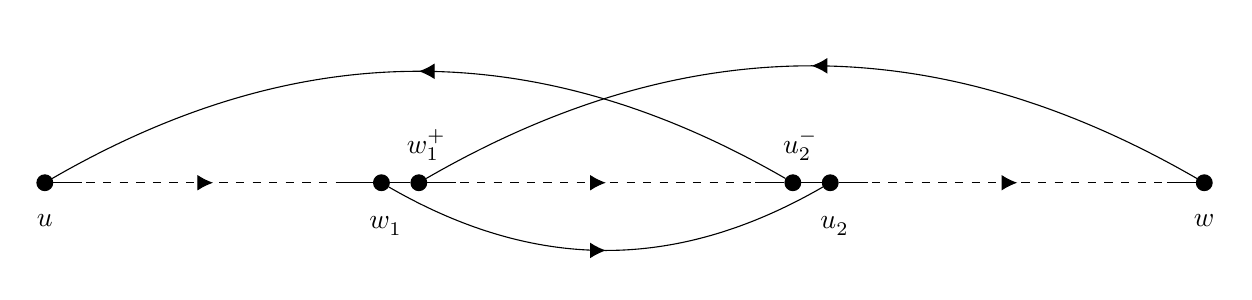
\begin{tikzpicture}[scale=0.95]

\node[vertex] (u) at  (0,0) {};
\node[vertex] (w1) at  (4.5,0) {};
\node[vertex] (w1p) at  (5,0) {};
\node[vertex] (u2m) at  (10,0) {};
\node[vertex] (u2) at (10.5,0) {};
\node[vertex] (w) at (15.5,0) {};

\draw (u) to (0.5,0);
\draw[arc,dashed] (u) to (w1);
\draw (4,0) to (w1);
\draw (w1) to (w1p);
\draw (w1p) to (5.5,0);
\draw[arc,dashed] (w1p) to (u2m);
\draw (9.5,0) to (u2m);
\draw (u2m) to (u2);
\draw (u2) to (11,0);
\draw[arc,dashed] (u2) to (w);
\draw (15,0) to (w);
\draw[arc] (w) to [bend right] (w1p);
\draw[arc] (u2m)  to [bend right] (u);
\draw[arc] (w1) to [bend right] (u2);

%\draw[line width=5, opacity=0.3, blue] (u) to (w1) to [bend right] (u2) to (w) to [bend right] (w1p) to (u2m) to [bend right] (u);

\node at (4.6,-0.5){$w_1^{\phantom+}$};
\node at (5.1,0.5){$w_1^+$};
\node at (10.1,0.5){$u_2^-$};
\node at (10.6,-0.5){$u_2^{\phantom-}$};
\node at (0,-0.5){$u$};
\node at (15.5,-0.5){$w$};

\end{tikzpicture}
\hspace{0.5cm}
\end{center}

\protect\caption{\label{fig:pseudorandom-hamiltonian-case-1}The case where the vertices
of $W_{1}$ precede the vertices of $U_{2}$. The horizontal line
through the center is $P$; the broken lines indicate subpaths.}
\end{figure}


Otherwise, each vertex of $U_{1}$ precedes each vertex of $W_{2}$.
Let $U_{12}$ contain the $k$ elements of $U_{1}$ furthest down
the path. Let $U_{11}$ be the set of vertices among the first $2k$
vertices of $P$ which have an arc to $U_{12}^{+}$. By the discussion
at the beginning of the proof, $\left|U_{11}\right|\ge k$. Similarly,
let $W_{21}$ contain the $k$ elements of $W_{2}$ first appearing
on the path, and let $W_{22}$ be the set of at least $k$ vertices
among the last $2k$ on $P$ which have an arc from $W_{21}^{-}$.
By the condition on $D$, there is an arc $w_{22}u_{11}$ from $W_{22}^{-}$
to $U_{11}^{+}$. By definition, there is $u_{12}\in U_{12}^{+}$
and $w_{21}\in W_{21}^{-}$ such that the arcs $u_{11}^{-}u_{12}$
and $w_{21}w_{22}^{+}$ are in $D$. We can piece everything together
to get a cycle on the vertices of $P$: start at $u_{11}$, move along
$P$ until $u_{12}^{-}$, then jump back to $u$. Move along $P$
until $u_{11}^{-}$, then take the shortcut to $u_{12}$. Continue
along $P$ to $w_{21}$, jump to $w_{22}^{+}$, continue to $w$,
jump back to $w_{21}^{+}$, and continue to $w_{22}$. From here there
is a shortcut back to $u_{11}$. See Figure \ref{fig:pseudorandom-hamiltonian-case-2}.

\begin{figure}[H]
\begin{center}
\hspace{0.5cm}
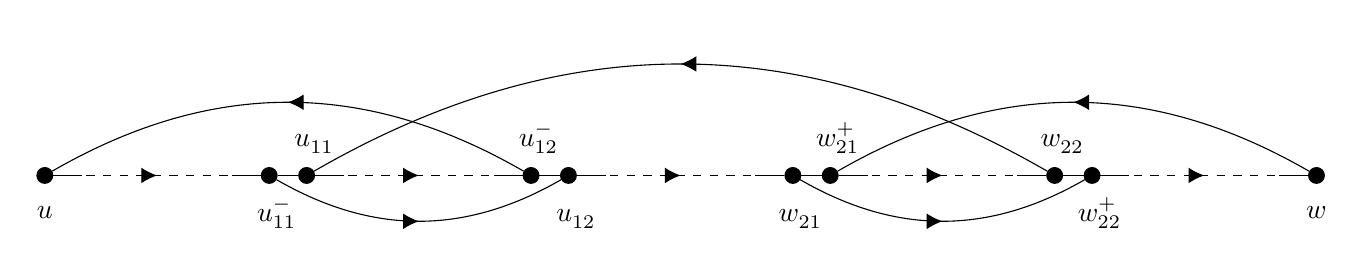
\begin{tikzpicture}[scale=0.95]

\node[vertex] (u) at  (0,0) {};
\node (up) at  (0.5,0) {};
\node (u11mm) at  (2.5,0) {};
\node[vertex] (u11m) at  (3,0) {};
\node[vertex] (u11) at  (3.5,0) {};
\node[vertex] (u12m) at  (6.5,0) {};
\node[vertex] (u12) at  (7,0) {};
\node[vertex] (w21) at  (10,0) {};
\node[vertex] (w21p) at  (10.5,0) {};
\node[vertex] (w22) at  (13.5,0) {};
\node[vertex] (w22p) at  (14,0) {};
\node[vertex] (w) at  (17,0) {};

\draw (u) to (0.5,0);
\draw[arc,dashed] (u) to (u11m);
\draw (2.5,0) to (u11m);
\draw (u11m) to (u11);
\draw (u11) to (4,0);
\draw[arc,dashed] (u11) to (u12m);
\draw (u12m) to (6,0);
\draw (u12m) to (u12);
\draw (u12) to (7.5,0);
\draw[arc,dashed] (u12) to (w21);
\draw (9.5,0) to (w21);
\draw (w21) to (w21p);
\draw (w21p) to (11,0);
\draw[arc,dashed] (w21p) to (w22);
\draw (13,0) to (w22);
\draw (w22) to (w22p);
\draw (w22p) to (14.5,0);
\draw[arc,dashed] (w22p) to (w);
\draw (16.5,0) to (w);
\draw[arc] (u12m) to [bend right] (u);
\draw[arc] (u11m)  to [bend right] (u12);
\draw[arc] (w21) to [bend right] (w22p);
\draw[arc] (w) to [bend right] (w21p);
\draw[arc] (w22) to [bend right] (u11);

%\draw[line width=5, opacity=0.3, blue] (u) to (w1) to [bend right] (u2) to (w) to [bend right] (w1p) to (u2m) to [bend right] (u);

\node at (0,-0.5){$u$};
\node at (3.1,-0.5){$u_{11}^-$};
\node at (3.6,0.5){$u_{11}^{\phantom-}$};
\node at (6.6,0.5){$u_{12}^-$};
\node at (7.1,-0.5){$u_{12}^{\phantom-}$};
\node at (10.1,-0.5){$w_{21}^{\phantom+}$};
\node at (10.6,0.5){$w_{21}^+$};
\node at (13.6,0.5){$w_{22}^{\phantom+}$};
\node at (14.1,-0.5){$w_{22}^+$};
\node at (17,-0.5){$w$};

\end{tikzpicture}
\hspace{0.5cm}
\end{center}

\protect\caption{\label{fig:pseudorandom-hamiltonian-case-2}The case where the vertices
of $U_{1}$ precede the vertices of $W_{2}$.}
\end{figure}

\end{proof}

\begin{proof}
[Proof of Lemma \ref{lem:pseudorandom-hamiltonian}]Fix a vertex $v$.
Let $U^{+}$ and $U^{-}$ be arbitrary $k$-subsets of $N^{+}\left(v\right)$
and $N^{-}\left(v\right)$ respectively. There is an arc from $U^{+}$
to $U^{-}$ which immediately gives a 3-cycle.

Next, let $W^{+}$ be the set of (fewer than $k$) vertices with no
arc into $U^{+}$, and similarly let $W^{-}$ be the set of vertices
with no arc from $U^{-}$. Now consider the induced digraph $D'$
obtained from $D$ by deleting $v$ and the vertices in $U^{+},U^{-},W^{+},W^{-}$.
Since we have removed fewer than $4k$ vertices, $D'$ satisfies the
conditions of Lemma \ref{lem:pseudorandom-hamiltonian} so has a Hamilton
cycle. In particular, for every $\ell$ satisfying $4\le\ell\le n-4k$,
there is a path $P_{\ell}=u_{\ell}\dots w_{\ell}$ in $D'$ of length
$\ell-4$. By construction, there is an arc from $U^{+}$ to $u_{\ell}$
and from $w_{\ell}$ to $U^{-}$, which we can combine with arcs to
and from $v$ to get a cycle of length $\ell$.

Finally, for every $\ell>n-4k$, arbitrarily delete vertices from
$D$ to obtain an induced digraph $D''$ with $\ell$ vertices which
satisfies the conditions of Lemma \ref{lem:pseudorandom-hamiltonian}.
Since $D''$ has a Hamilton cycle, $D$ has a cycle of length $\ell$.
\end{proof}

\begin{proof}
[Proof of Theorem \ref{thm:smoothed-pancyclic}]Consider the alternative
model where we add to $D$ each arc not in $D$ with independent probability
$p=2\beta\left(\alpha\right)/n$. By \cite[Corollary 1.16(i)]{JLR00},
it suffices to prove that $D''$ a.a.s. has a Hamilton cycle. In what
follows, we omit floor symbols and implicitly round to an integer
where appropriate.

If $A,B\subseteq V\left(D\right)$ are disjoint sets with $\left|A\right|=\left|B\right|=\alpha n/8$,
the probability that there are no arcs from $A$ to $B$ in $D''$
is at most
\[
\left(1-p\right)^{\left(\alpha n/8\right)^{2}}\le e^{-p\alpha^{2}n^{2}/64}=e^{-\beta\left(\alpha\right)\alpha^{2}n/32}.
\]
The number of choices of such pairs of disjoint sets $A,B$ is 
\[
{n \choose \alpha n/4}{\alpha n/4 \choose \alpha n/8}=O\left(\frac{1}{\sqrt{n}}e^{n\left(H\left(\alpha/4\right)+\alpha H\left(1/2\right)/4\right)}\right),
\]
where $H\left(\alpha\right)=-\alpha\log\alpha-\left(1-\alpha\right)\log\left(1-\alpha\right)$
(this can be proved with Stirling's approximation). By a union bound,
the probability that $D''$ does not satisfy the condition of Lemma
\ref{lem:pseudorandom-hamiltonian} is at most
\[
O\left(\frac{1}{\sqrt{n}}e^{n\left(H\left(\alpha/4\right)+\alpha H\left(1/2\right)/4-\beta\left(\alpha\right)\alpha^{2}n/32+o\left(1\right)\right)}\right).
\]
This converges to zero if $\beta\left(\alpha\right)$ is chosen to
be sufficiently large.\end{proof}
\begin{rem}
If we are only interested in Hamiltonicity, we can use Lemma \ref{lem:pseudorandom-hamiltonian}
directly in the proof of Theorem \ref{thm:smoothed-pancyclic}, which
gives a better constant $\beta\left(\alpha\right)$ than in \cite[Theorem 3]{BFM03}.
If we make the adjustment for undirected graphs mentioned in \ref{rem:constants},
then we also beat the corresponding constant in \cite[Theorem 1]{BFM03}
for large values of $\alpha$.
\end{rem}

\section{Hamiltonicity in tournaments}

I WILL REWRITE THIS INTRODUCTION LATER.

A \emph{tournament} is a directed graph obtained by assigning a direction
for each edge in a complete graph. A digraph is \emph{strongly connected}
if there is a directed path between any pair of vertices. It was proved
in \cite{MM62} that almost all tournaments are strongly connected,
in the sense that the proportion of tournaments on $n$ vertices that
are strongly connected converges to 1 as $n\to\infty$. Our preferred
interpretation of this fact is that a uniformly random tournament
is strongly connected with probability converging to 1 (\emph{asymptotically
almost surely}, or \emph{a.a.s.} for short).

It is not true that every sufficiently large tournament is strongly
connected. For example, a \emph{transitive} tournament (corresponding
to a linear order on the vertices) is never strongly connected. We
are interested in understanding how ``fragile'' such counterexamples
are, by asking how much a fixed tournament $T$ must be randomly perturbed
to make it strongly connected. Questions of this type are of particular
interest in the setting of \emph{smoothed analysis} of algorithms,
introduced in \cite{ST04}. In this setting, instead of considering
absolute worst-case inputs, we consider the ``approximate'' worst
case.

If $T$ is a transitive tournament, our question was effectively answered
in \cite[Section 3]{LRG96}: flipping each arc with probability $\omega\left(1/n\right)$
will result in a strongly connected tournament a.a.s., and a gentler
perturbation will not suffice.

Unsurprisingly, we find that transitive tournaments are a ``worst
case'', in that flipping a superlinear number of arcs suffices for
all $T$. We also find that the vertices in a transitive tournament
with only outgoing or only incoming arcs are a ``bottleneck'' for
strong connectivity, and a gentler random perturbation suffices for
tournaments which do not have such ``imbalanced'' vertices. Denote
the minimum indegree and outdegree of $T$ by $\delta^{-}\left(T\right)$
and $\delta^{-}\left(T\right)$ respectively, and let $\delta\left(T\right)=\min\left\{ \delta^{-}\left(T\right),\delta^{+}\left(T\right)\right\} $.
We prove the following theorem.
\begin{thm}
\label{thm:tournament}Consider a tournament $T$ with $n$ vertices
and $\delta\left(T\right)\ge d$. Independently designate each arc
as ``random'' with probability $p$ satisfying $np\left(d+1\right)\to\infty$,
then choose the orientations of the chosen edges independently and
uniformly at random. The resulting perturbed tournament $P$ a.a.s.
has $t$ arc-disjoint Hamilton cycles, for any fixed $t$.
\end{thm}
This theorem is sharp, in the sense that if we do not have $np\left(d+1\right)\to\infty$
then $P$ might not be a.a.s. Hamiltonian. To see this, consider a
``transitive cluster-tournament'' $T$ on $n=rk$ vertices defined
as follows. Let $R$ be a regular tournament on $2d+1$ vertices (this
means the indegree and outdegree are equal for each vertex). To construct
$T$, start with $r$ disjoint copies $R_{1},\dots,R_{r}$ of $R$,
then put an arc from $v$ to $w$ for every $v\in R_{i}$, $w\in R_{j}$
with $i<j$. In order for the perturbed tournament $P$ to be Hamiltonian,
there must be an arc entering $R_{1}$, so one of the $O\left(n\left(d+1\right)\right)$
arcs exiting $R_{1}$ must be resampled. This will not happen a.a.s.
unless $pn\left(d+1\right)\to\infty$.
\begin{rem}
\label{rem:different-models}Theorem \ref{thm:tournament} is stated
with a particular type of seemingly complicated random perturbation.
The reason we have chosen this model is because it is ``monotone''
in that performing two small perturbations is the same as performing
one big perturbation, and because it has convenient independence properties.
However, the result is not sensitive to the model of perturbation.
NEED TO ELABORATE.
\end{rem}

\subsection{Proof of Theorem \ref{thm:tournament}}

There are several seemingly different conditions that are equivalent
to Hamiltonicity for tournaments (see \cite[Chapters 2-3]{Moo68}).
A tournament is strongly connected if and only if it is irreducible
(cannot be divided into two partitions with all arcs between the two
partitions in the same direction), if and only if it is Hamiltonian
(has a directed cycle containing all the vertices), if and only if
it is pancyclic (contains cycles of all lengths). It was more recently
proved in \cite{Pok14} that if a tournament is $t$-strongly connected
(it remains strongly connected after the deletion of $t-1$ vertices),
then it has $O\left(\sqrt{t}\right)$ arc-disjoint Hamilton cycles.
Theorem \ref{thm:tournament} then implies that $P$ contains $q$
arc-disjoint Hamilton cycles for $q=O\left(1\right)$.

We therefore prove that $P$ is $t$-strongly connected. The idea
of the proof is to choose a set $S$ of $t$ vertices with a large
indegree and outdegree. Then we show that with high probability almost
every vertex has many paths to and from each vertex in $S$.
\begin{lem}
\label{lem:extreme-indegree-bound}In any tournament, there are less
than $k$ vertices with indegree (respectively outdegree) less than
$\left(k-1\right)/2$.\end{lem}
\begin{proof}
The sum of indegrees (respectively outdegrees) of a tournament on
$k$ vertices is ${k \choose 2}$, because each arc contributes 1
to this sum. Therefore in every set of $k$ vertices of a tournament,
there is a vertex of outdegree (indegree) at least $\left(k-1\right)/2$
in the induced tournament.
\end{proof}
It follows from Lemma \ref{lem:extreme-indegree-bound} that the set
of all vertices with indegree (respectively outdegree) less than $n/6$
has size smaller than $n/3$. So, there are at least $n/3$ vertices
with indegree and outdegree at least $n/6$. Since $t=O\left(1\right)=o\left(n/6\right)$,
there is a set $S$ of $t$ such vertices.
\begin{lem}
\label{lem:preserve-degree}If a vertex $v$ has outdegree (respectively
indegree) $k$ in $T$, then it has outdegree (respectively indegree)
at least $k/3$ in $P$, with probability $e^{-\Omega\left(\sqrt{n}\right)}$
uniformly over $k$.\end{lem}
\begin{proof}
We only prove the statement where $v$ has outdegree $k$; the indegree
case is identical. If $k=0$ the lemma is trivial, so assume $k\ge1$.
First consider the cases where $k>\sqrt{n}$ or $p<1/\sqrt{n}$. There
are $k$ arcs pointing away from $v$ in $T$; let $X$ be the number
of those arcs that are changed by the perturbation. Since $X\in\Bin\left(k,p/2\right)$,
a Chernoff bound gives
\[
\Pr\left(X>2k/3\right)\le\Pr\left(X-\E X>k/6\right)\le e^{-\Omega\left(k^{2}/\E X\right)}=e^{-\Omega\left(\sqrt{n}\right)}.
\]
That is, with the required probability, $k/3$ of the original out-neighbours
survive the perturbation.

Otherwise (for large $n$), there is a set of $n/2$ arcs pointing
towards $v$ in $T$. Let $Y$ be the number of these arcs that are
changed by the perturbation, so $Y\in\Bin\left(n/2,p/2\right)$ with
$\E Y\ge\sqrt{n}/2$. Then,
\[
\Pr\left(Y<k/3\right)\le\Pr\left(X-\E Y<-\E Y/3\right)\le e^{-\Omega\left(\sqrt{n}\right)},
\]
so with the required probability, $k/3$ new out-neighbours are added
by the perturbation.\end{proof}
\begin{lem}
\label{lem:path-from-home}Suppose $w$ has outdegree (respectively
indegree) at least $n/6$, and $v\ne w$ is a vertex with indegree
(respectively outdegree) at least $k$. Then with probability $1-e^{-\Omega\left(\sqrt{n}\right)}-e^{-\Omega\left(np\left(k+1\right)\right)}$
(uniformly over $k$), there are $t'=3t$ internally vertex-disjoint
paths of length at most 3 from $w$ to $v$ (respectively from $v$
to $w$).\end{lem}
\begin{proof}
We will only prove the statement where $v$ has indegree at least
$k$; the other case is identical. By independence, we can condition
on the outcome of the perturbation on individual arcs. Condition on
the outcome for all arcs adjacent to $w$, and let $N_{P}^{+}\left(w\right)$
be the set of vertices to which there is an arc from $w$ in $P$.
By Lemma \ref{lem:preserve-degree}, we can assume $\left|N_{P}^{+}\left(w\right)\right|\ge n/18$.

We first prove the lemma for the case where $k\le12t'$. There are
at least $n'=n/18-1$ arcs between $N_{P}^{+}\left(w\right)$ and
$v$, each of which will be pointing towards $v$ in $P$ with independent
probability at least $p/2$. Let $Z\in\Bin\left(n',p/2\right)$. The
probability that less than $t'$ arcs will point from $N_{P}^{+}\left(w\right)$
to $v$ in $P$ is at most
\[
\Pr\left(Z<t'\right)\le e^{-\Omega\left(\E Z-t'\right)}=e^{-\Omega\left(np\right)}=e^{-\Omega\left(np\left(k+1\right)\right)}.
\]
So, with the required probability there are $t'$ suitable length-2
paths from $w$ to $v$.

We can now assume $k>12t'$. Condition on the result of the perturbation
for the arcs adjacent to $v$. Let $N_{P}^{-}\left(v\right)$ be the
set of vertices from which there is an edge into $v$ in $P$; by
Lemma \ref{lem:preserve-degree}, we can assume $\left|N_{P}^{-}\left(v\right)\right|\ge k/3$.

Now, if $\left|N_{P}^{+}\left(w\right)\cap N_{P}^{-}\left(v\right)\right|\ge t'$
then there are $t'$ disjoint length-2 paths from $w$ to $v$ and
we are done. So we can assume $U^{+}=N_{P}^{+}\left(w\right)\backslash\left(N_{P}^{-}\left(v\right)\cup\left\{ v\right\} \right)$
has at least $n'=n/18-t'-1$ vertices, and $U^{-}=N_{P}^{-}\left(v\right)\backslash\left(N_{P}^{+}\left(w\right)\cup\left\{ w\right\} \right)$
has at least $k'=k/6-t'-1$ vertices (note $k'\ge t'$ by assumption).

Now, we would like to show that with the required probability there
is a set of $t'$ independent arcs from $U^{+}$ into $U^{-}$ in
$P$, which will give $t'$ suitable length-3 paths. Partition $U^{+}$(respectively
$U^{-}$) into subsets $U_{1}^{+},\dots,U_{t'}^{+}$ (respectively
$U_{1}^{-},\dots,U_{t'}^{-}$), such that each $\left|U_{1}^{+}\right|>n'/\left(2t'\right)$
and each $\left|U_{1}^{-}\right|>k'/\left(2t'\right)$. For each $i$,
the probability that there is no arc from $U_{i}^{+}$ into $U_{i}^{-}$
after the perturbation is at most
\[
\left(1-p/2\right)^{n'k'/\left(4t'\right)}\le e^{-\Theta\left(np\left(k+1\right)\right)},
\]
so with the required probability there a set of $t'$ suitable independent
arcs, each between a pair $U_{i}^{+},U_{i}^{-}$.\end{proof}
\begin{lem}
\label{lem:lots-of-paths}Fix some $w\in S$. In $P$, there are a.a.s.
$t$ disjoint paths from $w$ to each other vertex (respectively,
from each other vertex to $w$).\end{lem}
\begin{proof}
We only prove there are paths from $w$ to each other vertex; the
reverse case is identical. If there are $3t$ disjoint paths of length
at most 3 from $w$ to $v$ then we say $v$ is \emph{safe}. It follows
from Lemma \ref{lem:path-from-home} that a vertex with indegree $k$
is safe with probability $1-e^{-\Omega\left(\sqrt{n}\right)}-e^{-\Omega\left(np\left(k+1\right)\right)}$.

By Lemma \ref{lem:extreme-indegree-bound}, there are at most $\left(2d+1\right)$
vertices with outdegree $d$, and the vertex with the $2k$th smallest
outdegree has outdegree at least $k-1$. Let $Q$ be the set of non-safe
vertices, and note
\begin{align*}
\E\left|Q\right| & =\left(2d+1\right)e^{-\Omega\left(np\left(d+1\right)\right)}+\sum_{k=d+1}^{n}2e^{-\Omega\left(np\left(k+1\right)\right)}+ne^{-\Omega\left(\sqrt{n}\right)}\\
 & =e^{-\Omega\left(np\left(d+1\right)\right)}\left(O\left(d+1\right)+\frac{1}{1-e^{-\Omega\left(np\right)}}\right)+o\left(1\right)\\
 & =e^{-\Omega\left(np\left(d+1\right)\right)}O\left(d+1\right).
\end{align*}
where we have used the geometric series formula, the inequality $1-e^{-x}\ge\left(x\land1\right)/2$
(for positive $x$) and the fact that $d+1=\Omega\left(1\right)$.

By Markov's inequality, a.a.s. $\left|Q\right|\le\sqrt{e^{-\Omega\left(pn\left(d+1\right)\right)}}O\left(d+1\right)=o\left(d+1\right)$.
If $d\le4t$ then $\left|Q\right|=0$ for large $n$. Otherwise, for
large $n$, $\left|Q\right|\le3d$, so every vertex $v\in Q$ has
$3t$ safe neighbours $v_{1},\dots,v_{3t}$. Now, fix a maximal set
$M$ of disjoint paths from $w$ to $v$. If $\left|M\right|<t$ then
the paths in $M$ collectively use less than $3t$ vertices other
than $t$, so there is some $v_{i}$ not in any path of $M$, and
there is some path from $w$ to $v_{i}$ that does not contain any
vertex of $M$. But then $w\dots v_{i}v$ is a path from $w$ to $v$
disjoint with every path in $M$, contradicting maximality.
\end{proof}
It follows from Lemma \ref{lem:lots-of-paths} that a.a.s. every vertex
outside $S$ has $t$ disjoint paths to and from every vertex in $S$.
If we delete $t-1$ vertices, then there is at least one vertex $w$
of $S$ remaining, and $w$ has least one path to and from every other
vertex. That is, $P$ is strongly connected. (In fact, we have also
proved that $P$ has diameter at most 8).

\bibliographystyle{amsalpha}
\bibliography{references}

\end{document}
